\begin{figure*}[t!]
    \centering
    \begin{minipage}{0.34\linewidth}
    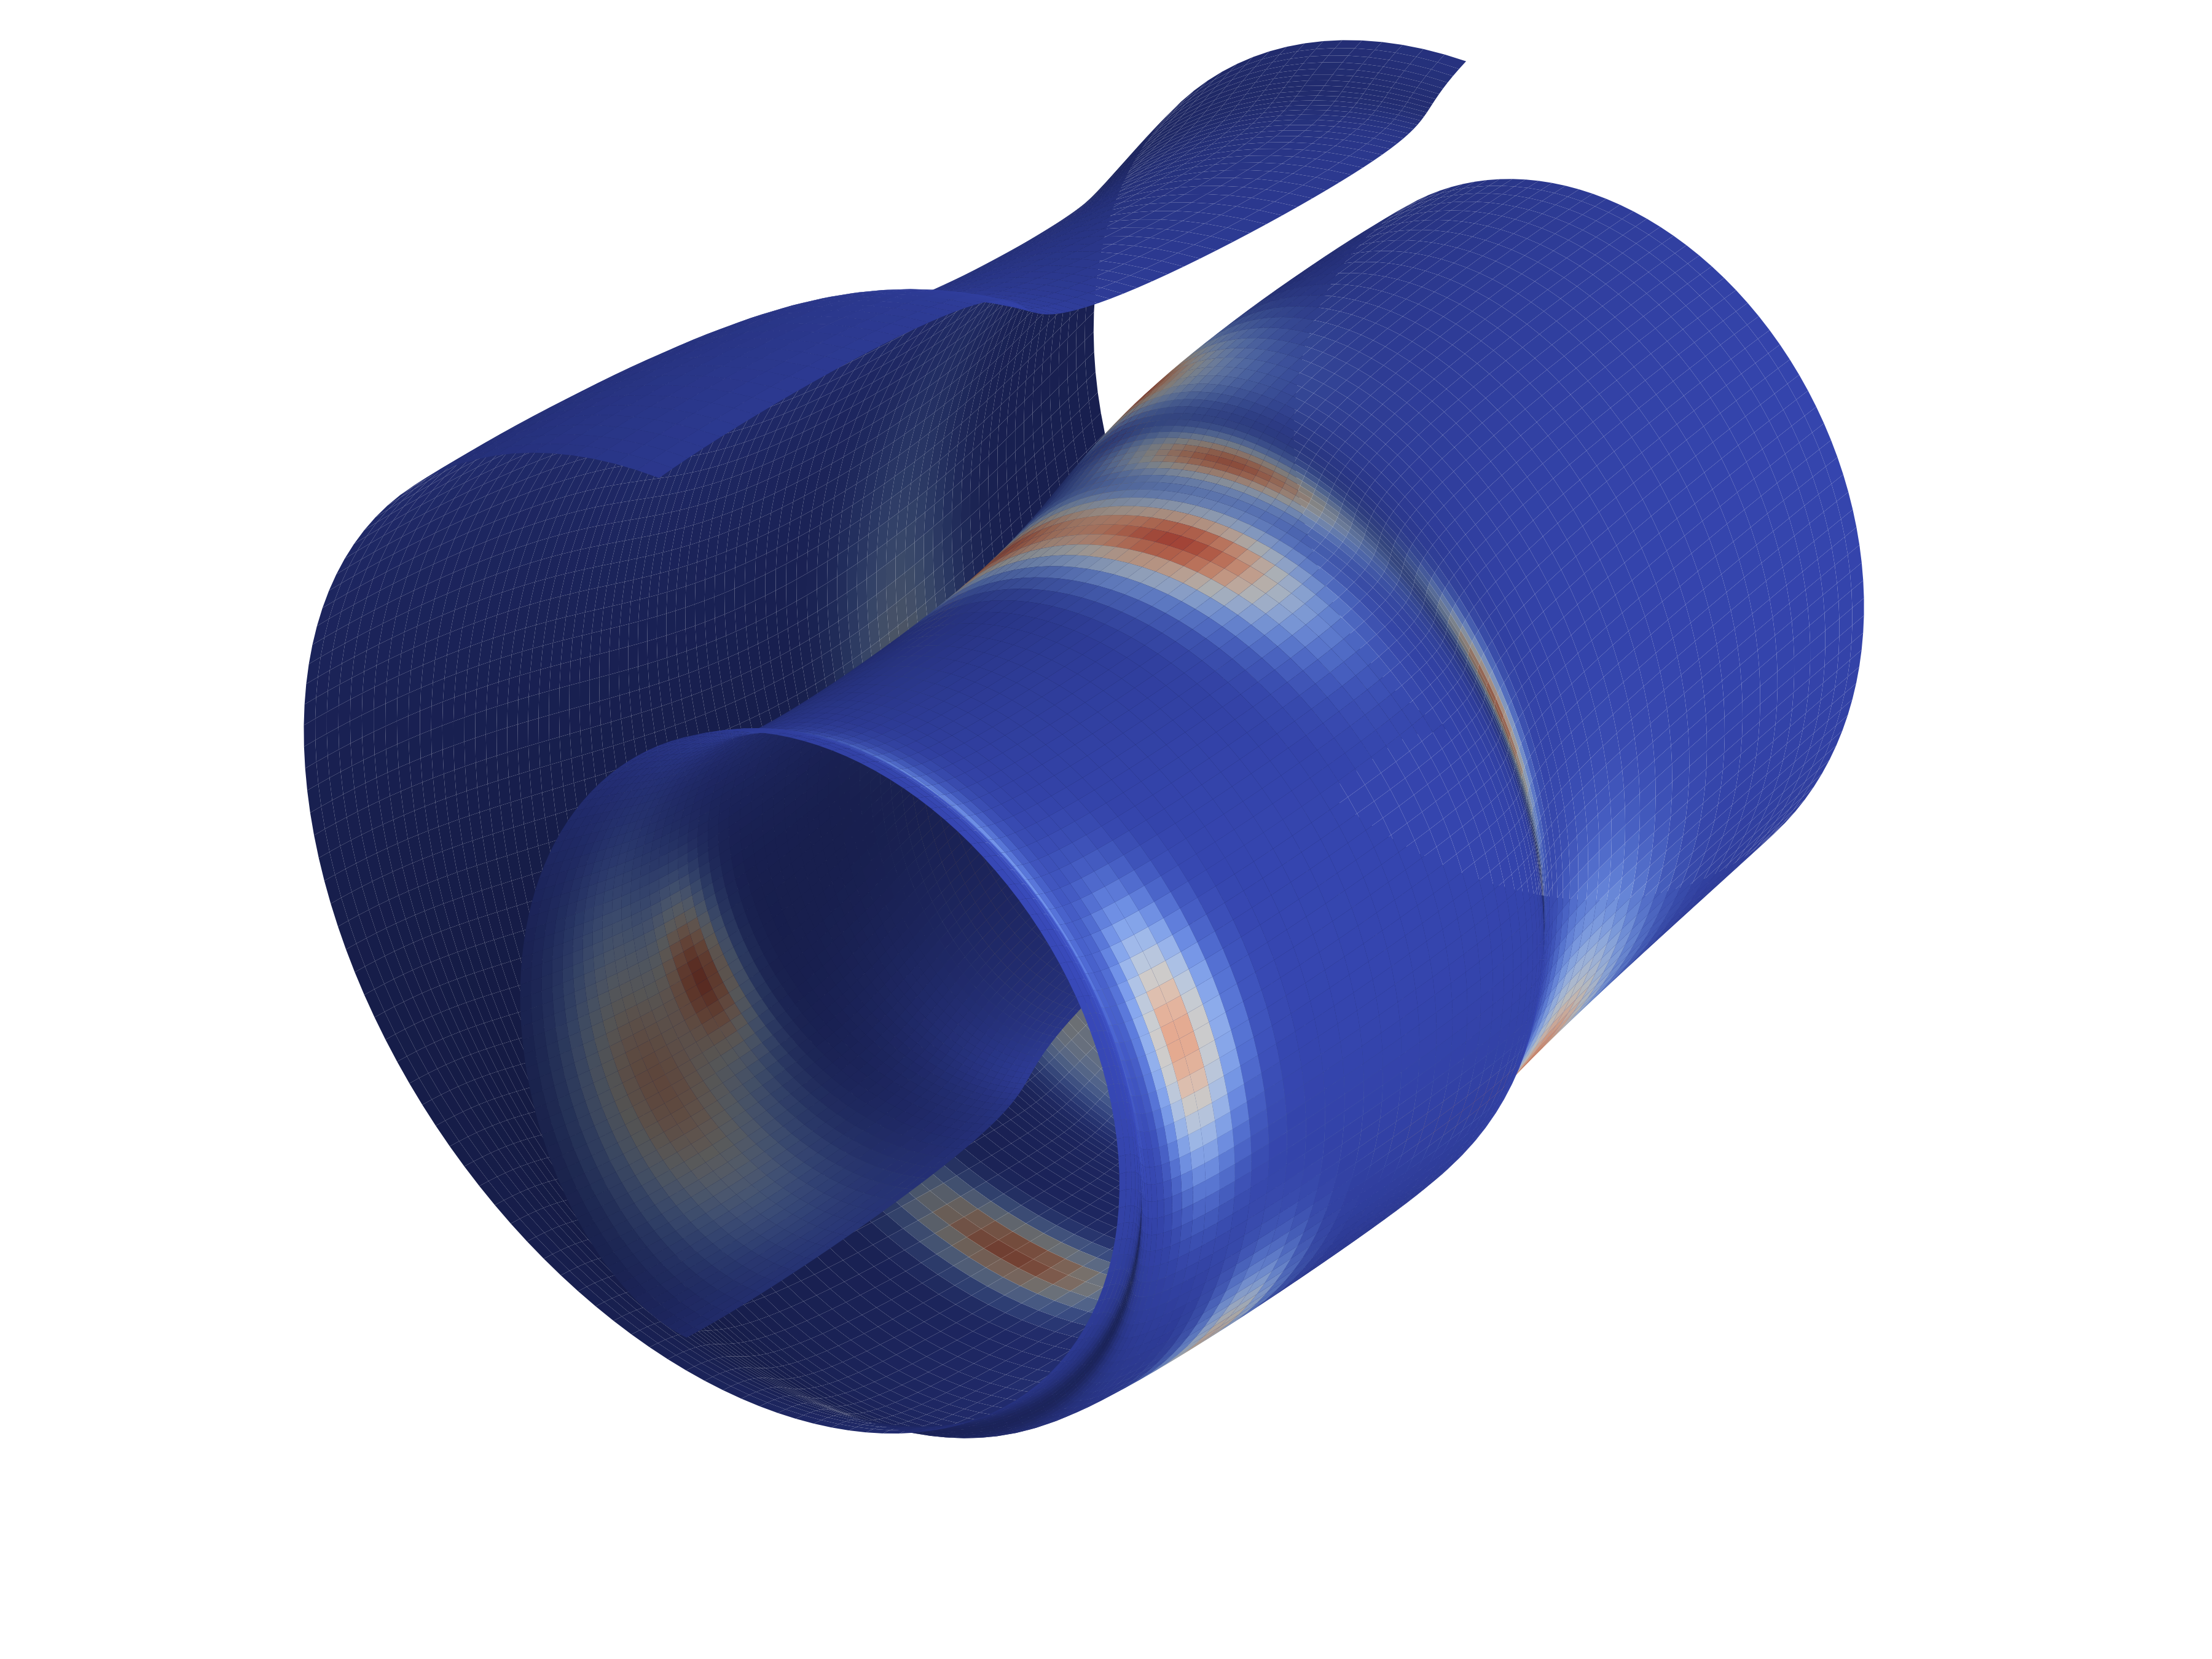
\includegraphics[width=\linewidth]{toy_figures/teaser/teaser_manifold_0.png}
    \end{minipage}
    \begin{minipage}{0.05\linewidth}
    \hspace{-0.4cm}{\Large $\underset{\rightarrow}{f_{\vtheta}}$}
    \end{minipage}
    \begin{minipage}{0.6\linewidth}    \hspace{-0.3cm}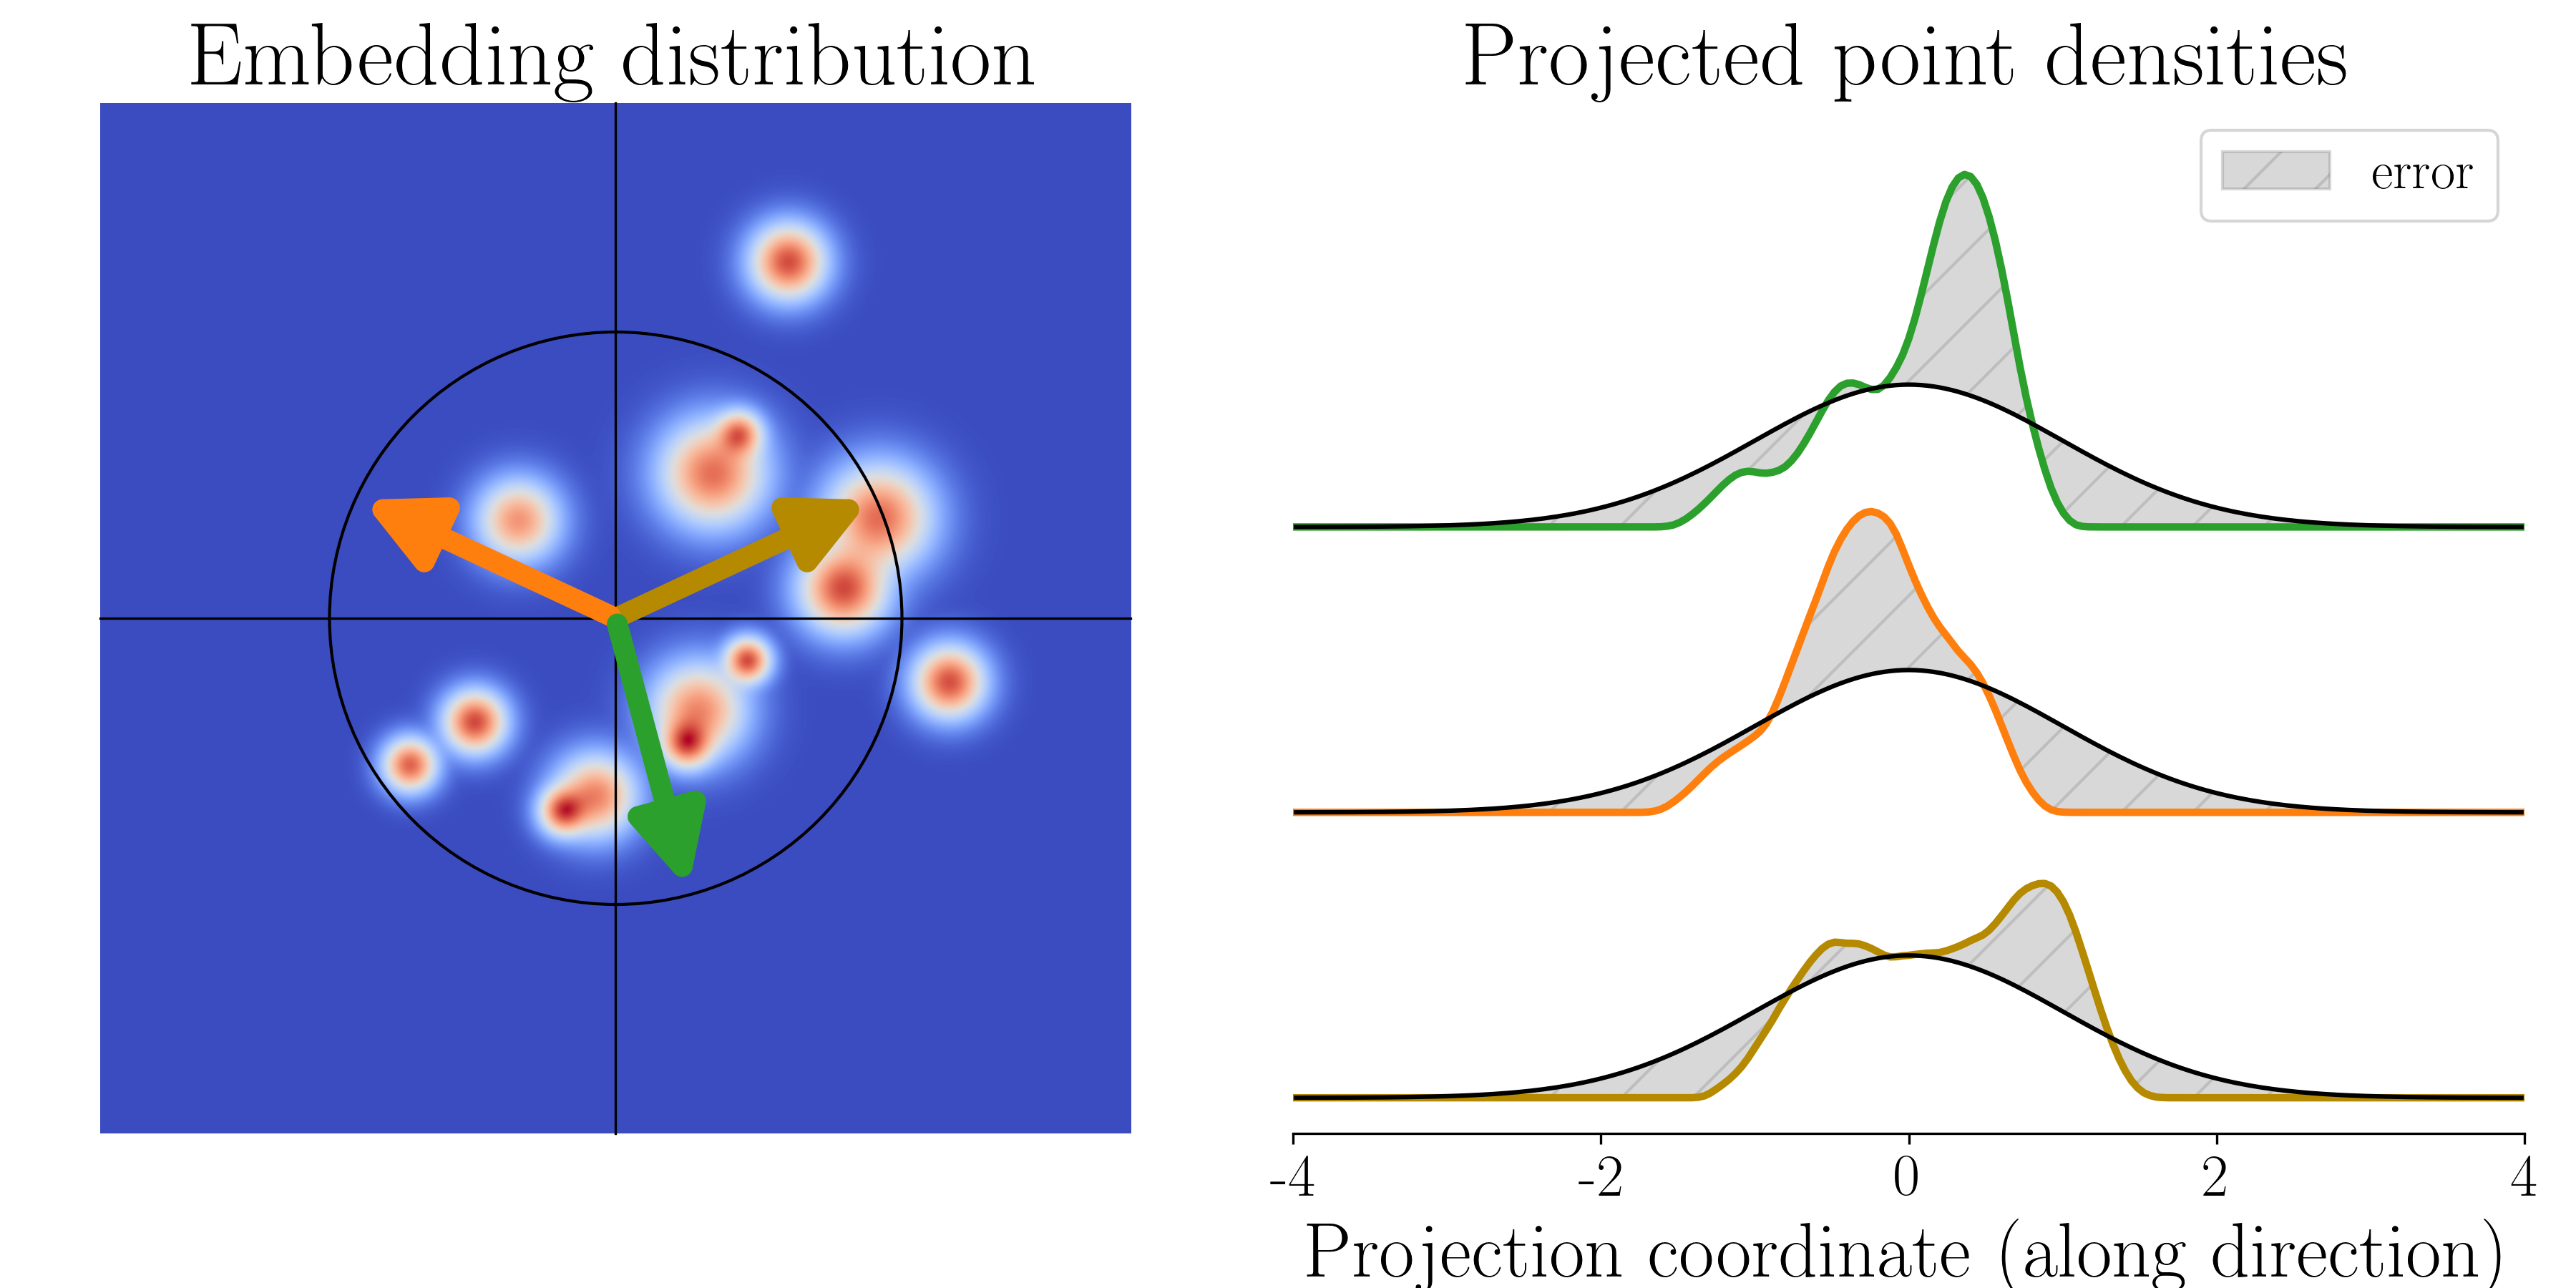
\includegraphics[width=\linewidth]{toy_figures/teaser/teaser_manifold_1.png}
    \end{minipage}
    \caption{ \textbf{Sketched Isotropic Gaussian Regularization (SIGReg):}~Given some arbitrary input data with density $p_{x}$ with support that may or may not lie on a manifold ({\bf left}), a Deep network (DN) encoder ($f_{\vtheta}$) produces embeddings $\vz=f_{\vtheta}(\vx)$ with some distribution $\vz \sim p_{z}$ ({\bf middle}). Our proposed Backward Cramér-Wold Statistics (\cref{sec:bcs}) objective pushes $p_z$ to match a target distribution $p_t$ by projecting the embeddings along $1d$ directions ({\bf middle, arrows}) and enforcing that the univariate densities ({\bf right, colored lines}) match the distribution of $p_t$, projected along the same directions. Any popular statistical test (provided in \cref{sec:tests}) can assess the goodness-of-fit--in practice we argue for characteristic function tests (\cref{sec:CF_better}). By using SIGReg with $p_t$ isotropic Gaussian ({\bf right, black lines}), we introduce a lean and provably optimal (\cref{sec:gaussian}) JEPA, coined LeJEPA, free of numerous heuristics and able to produce competitive performances (\cref{sec:lejepa,sec:experiments}).}
    \label{fig:bcs_teaser}
\end{figure*}


\section{Introduction}
\label{sec:intro}


Learning manipulable representations of the world and its dynamics is a long‑standing question in AI, with roots dating back centuries ago \citep{von1867handbuch,tolman1948cognitive,gregory1980perceptions,sutton1991dyna,friston2010free}. Across domains, e.g., image recognition, robotics, physics, space exploration, the unifying question is {\em how to learn an organized and actionable high‑dimensional embedding space from observations?} Using Deep Networks--parameterized nonlinear operators $f_{\vtheta}$--to map observations to embeddings is a standard first piece of that puzzle \citep{lecun2015deep,goodfellow2016deep}. The second, less standardized, piece of that puzzle is {\em how to train $f_{\vtheta}$}. Joint-Embedding Predictive Architectures (JEPAs) suggest training $f_{\vtheta}$ by maximizing predictive agreement between the embeddings of semantically related {\em views} \citep{bromley1993signature,lecun2022path,balestriero2023cookbook}. Views can come in two forms: transformations or corruptions.  They can involve masking, cropping, blurring, temporal or spatial translations, geometric or photometric transformations, viewpoint changes, views from different sensor modalities, etc. The supervised forms involve human-produced components such as image-caption pairs, text-code pairs, etc \citep{tian2020makes}. In any case, views are expected to share some degree of semantic relationship to allow the prediction task to align $f_{\vtheta}$'s embeddings towards the underlying knowledge present in the data.



Alas, JEPA's prediction task admits failure modes, such as representation collapse, where $f_{\vtheta}$ maps all inputs to 
nearly identical embeddings ({\em complete collapse}) or to a low-dimensional subspace 
({\em dimensional collapse}) \citep{jing2021understanding}\citep{jing2021understanding,cosentino2022toward,balestriero2022contrastive}. To mitigate such shortcut solutions, state‑of‑the‑art recipes rely on heuristics--stop‑gradient \citep{chen2020simple}, asymmetric view generation \citep{wang2022importance}, teacher–student networks with carefully tuned EMA schedules \citep{caron2021emerging,tian2021understanding}, explicit normalization and whitening layers \citep{ermolov2021whitening,chen2021empirical}--and a delicate balance of hyperparameters. As a result, today's JEPA training is brittle and most research has shifted toward scaling data \citep{vo2024automatic}, models \citep{fan2025scaling} and even post-training \cite{rodas2025diet} while leaving the theoretical foundations of JEPAs largely unexplored.


Our study proposes to break that cycle by questioning some of the fundamental design principles underpinning JEPAs. That introspection will start by asking {\em what are the necessary conditions that JEPAs should abide by?} Those minimal conditions will then act as {\em axioms} for us to design a novel and lean JEPA. We identify two axioms: (i) solving the prediction task while (ii) enforcing an isotropic Gaussian distribution of the embeddings (\cref{sec:gaussian}). While (i) follows standard practice \citep{balestriero2022contrastive}, we introduce  in \cref{sec:bcs} a novel  distribution matching objective--Sketched Isotropic Gaussian Regularization (SIGReg)--to enforce (ii). The use of SIGReg not only removes the need for the numerous heuristics previously employed to prevent representation collapse, but SIGReg also exhibits favorable scaling properties as its {\em memory and computational complexity is linear in dimension and sample size}. Crucially, SIGReg's isotropic Gaussian enforcement solves the collapsed shortcut solution and provably minimizes the model's expected risk over the space of downstream tasks to be encountered post-training. The resulting JEPA solution--coined Latent-Euclidean JEPA (LeJEPA)--is introduced in \cref{sec:lejepa}. Beyond theoretical optimality, LeJEPA offers numerous benefits such as (i) provable statistical guarantees, (ii) removal of heuristics such as teacher-student networks, (iii) linear memory and computational complexity, and most importantly (iv) a unified design with a single trade-off parameter that works out of the box across datasets, architectures and scales (see \cref{sec:experiments}). We summarize our contributions below.

{\bf Contribution 1: We prove the optimal embedding distribution for foundation models.}~We 
establish that the isotropic Gaussian uniquely minimizes downstream prediction risk across 
broad task families. In \cref{sec:gaussian}, we derive this result rigorously for both 
linear (\cref{sec:linear_probing}) and nonlinear probes (\cref{sec:nonlinear_probing}), 
providing the first principled answer to what distribution $f_{\vtheta}$'s embeddings 
should follow. This theoretical result transforms JEPA design from heuristic exploration 
to targeted optimization.
{\bf Contribution 2: We introduce SIGReg, a distribution matching objective that uniquely 
combines provable correctness with computational efficiency at scale.}~We present {\em 
Sketched Isotropic Gaussian Regularization} (SIGReg), a novel objective that enforces 
distributional alignment via random projections and characteristic-function matching 
(\cref{sec:bcs,fig:bcs_teaser}). SIGReg provides statistical guarantees 
(\cref{sec:general_test,sec:tests}) while achieving linear complexity and bounded 
gradients—a combination that existing distribution matching methods do not offer. 
Critically, its projection-based construction defeats the curse of dimensionality 
(\cref{sec:dimension}), making it both theoretically sound and practically efficient 
for high-dimensional embeddings.


{\bf Contribution 3: We design LeJEPA, a statistically optimal JEPA that eliminates 
collapse by construction.}~By combining JEPA's predictive objective with SIGReg targeting 
the isotropic Gaussian, we introduce {\em LeJEPA}—Latent-Euclidean JEPA 
(\cref{sec:lejepa}). LeJEPA requires only a single hyperparameter, 
eliminates representational collapse without stop-gradients or teacher-student 
architectures, and transfers across architectures and datasets without hyperparameter 
tuning. This demonstrates that principled theory directly yields practical simplicity.

{\bf Contribution 4: We validate LeJEPA at scale across diverse architectures and 
establish in-domain pretraining as viable.}~Our experiments (\cref{sec:experiments}) 
span ViTs, ConvNeXts, ResNets, MaxViTs, and Swin Transformers at scales approaching 
1 billion parameters, where LeJEPA matches or exceeds state-of-the-art methods while 
maintaining training simplicity and robustness. Critically, on domain-specific datasets 
(Galaxy10, Food101), LeJEPA outperforms DINOv2-based transfer learning when pretrained 
directly on target data. This challenges the transfer learning paradigm and demonstrates 
that principled SSL can unlock effective in-domain pretraining—previously considered 
impractical for small datasets.